Emando zit in het BizSpark programma van Microsoft. Vanuit BizSpark kunnen alle ontwikkeltools gratis gebruikt worden en Emando leunt dan ook op Microsoft technologie. Onderstaande methodologieën kunnen eenvoudig geïntegreerd worden in de ontwikkelomgeving Visual Studio. We zullen niet afwijken van de methodologieën die Emando nu al gebruikt, omdat ons deze omgeving wordt aangeboden en om onderhoudbaarheid in de toekomst te garanderen.

\section{Scrum}
In overleg met de opdrachtgever is er gekozen voor een Scrum aanpak voor het project. Scrum is een flexibele manier om software te ontwikkelen, zie ook Figuur~\ref{fig:scrum-proces}. Hierbij gaan we werken in een multidisciplinair team waarmee we in korte sprints, met een vaste lengte van tien werkdagen, werkende software opleveren en geleidelijk stabiele functionaliteit toe voegen. Een Scrum aanpak heeft als voordeel dat na iedere sprint er een werkend product af is, waarna de eisen en doelstellingen gemakkelijk bijgesteld kunnen worden. Met Scrum kunnen na de gebruikerstest, halverwege het project, de doelstellingen bijgesteld worden aan de hand van de uitkomst van deze test. Door deze agile methode toe te passen sluit het eindproduct altijd zo goed mogelijk aan op de wensen van de opdrachtgever en de end-users.

\begin{figure}[H]
  \begin{center}
    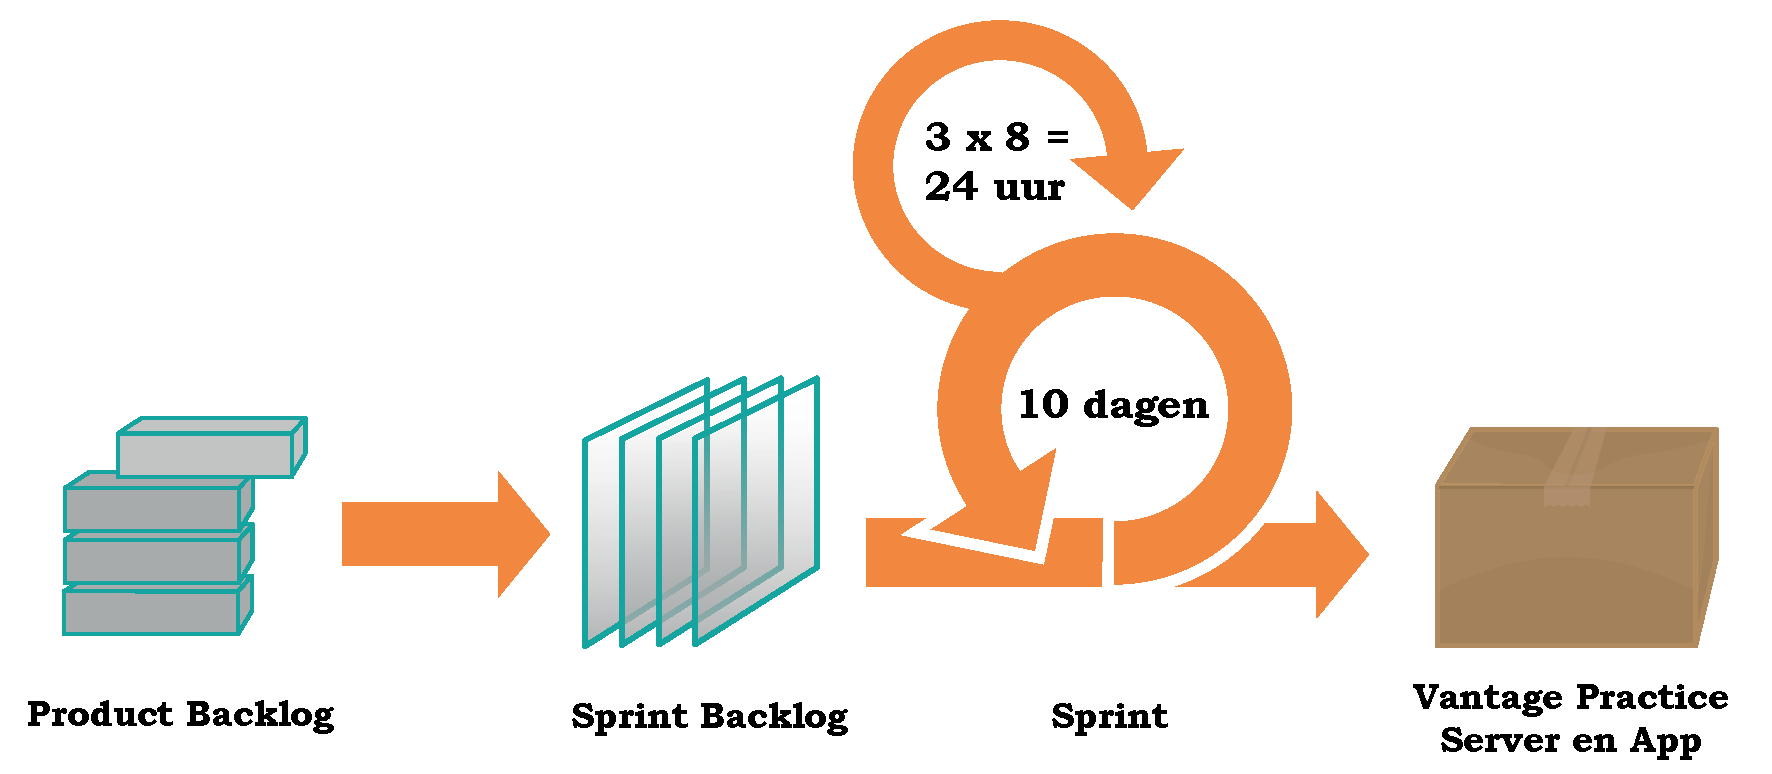
\includegraphics[width=0.8\textwidth]{style/images/Scrum}
  \end{center}
  \caption{Overzicht van het Scrum proces}
  \label{fig:scrum-proces}
\end{figure}

Aan het begin van het project is een lijst met Product Backlog items opgesteld. Deze items representeren de globale functionaliteiten van de applicatie en krijgen een teamlid toegewezen als verantwoordelijke. Voor elke sprint wordt bepaald welke van deze Backlog items er in de tien dagen-durende sprint geïmplementeerd zullen worden. Elk Backlog item bevat een aantal taken die voltooid moeten worden om het Backlog item af te krijgen. Aan deze taken wordt een aantal uren toegekend en vervolgens worden de taken verdeeld over de drie teamleden, afhankelijk van ieders expertise en de hoeveelheid beschikbare uren.

\section{Stand up meetings}
Om het overzicht binnen het project te waarborgen, zullen er iedere werkdag aan het begin van de dag stand up meetings met alle projectleden plaatsvinden. Bij deze stand up meetings wordt kort besproken waar momenteel aan gewerkt wordt, in hoeverre dit nog op schema ligt en waar de uitdagingen liggen voor de komende dagen. De opdrachtgever is ook minstens twee keer per week aanwezig bij deze meetings.

\section{\acl{tfs}}
Emando gebruikt \ac{tfs} voor het versiebeheer van broncode, het bijhouden van het ontwikkelproces, het tracken van issues en het visualiseren van de voortgang in projecten. De gemakkelijke integratie van \ac{tfs} met Visual Studio zorgt ervoor dat taken gemakkelijk toegewezen kunnen worden aan teamleden, waarna zij deze kunnen openen en hiermee aan de slag kunnen binnen Visual Studio. De status van deze items kan zowel vanuit Visual Studio als online aangepast worden en bij het afvinken van items kunnen deze gekoppeld worden aan versie nummers, zodat deze achteraf makkelijk vindbaar zijn. Daarnaast bestaat er een handig overzicht, te zien in Figuur~\ref{fig:scrum-board}, waarin in een oogopslag de status van alle taken bekeken kan worden.

\begin{figure}[H]
  \begin{center}
    \includegraphics[width=0.8\textwidth]{style/images/screenshots/ScrumBoard}
  \end{center}
  \caption{Overzicht van de activiteiten op het Scrum Board in \ac{tfs}}
  \label{fig:scrum-board}
\end{figure}

Ook zorgt de visualisatie van de zogenaamde `burndown', zoals in Figuur~\ref{fig:scrum-burndown}, van het project voor een inzichtelijke manier, waarbij de opdrachtgever in een handomslag de voortgang van het project in kan zien. Daarnaast biedt \ac{tfs} inzicht in de tijd die ieder issue en backlog item kost, hetgeen een goede indicatie is voor de scrum sprint. 

\begin{figure}[H]
  \begin{center}
    \includegraphics[width=0.6\textwidth]{style/images/screenshots/Burndown}
  \end{center}
  \caption{Burndown grafiek van Sprint 3 in \ac{tfs}}
  \label{fig:scrum-burndown}
\end{figure}

\subsection{Verantwoordelijkheden}
Samenhangend met de taakverdeling, hebben wij er voor gekozen om aan ieder backlog item een verantwoordelijke toe te kennen. Door de verantwoordelijkheden duidelijk te maken binnen het project, is het altijd duidelijk wie van welke functionaliteit kennis heeft en weet hoe de voortgang hiervan is. Hiermee is het ook mogelijk om slechts met een deel van de teamleaden en de opdrachtgever implementatie details door te spreken. Binnen \ac{tfs} is het mogelijk om de verantwoordelijkheden van taken en verantwoordelijkheden toe te kennen aan personen.

\subsection{Taakverdeling}
Om overlap van werk en functionaliteiten te voorkomen hebben we er voor gekozen om iedere functionaliteit uit te splitsen in verschillende backlog items en deze op hun beurt weer uit te splitsen in verschillende taken. Door deze taken klein te houden, is het makkelijker om de precieze invulling van functionaliteiten te definiëren. Daarnaast heeft dit als voordeel dat kleine taken sneller af zijn dan grote taken, waardoor de burndown van het project accurater is.

In grove lijnen ziet de verantwoordelijkheid en taak verdeling er als volgt uit:
\begin{enumerate}
\item Patrick van Hesteren: Back-end en Cloud
\item Hylke Visser: Grafische User Interface en Testen
\item Herman Banken: Applicatie en SignalR
\end{enumerate}

\section{Code Reviews}
Om de kwaliteit van het project te kunnen waarborgen, is voor de back-end van het project gekozen om te werken met Code Reviews. Omdat de back-end de core van het project vormt en tevens in de Cloud draait (waardoor er directe kosten zijn verbonden aan de kwaliteit van de code) is het belangrijk dat deze efficiënt en naar behoren werkt. Bij het implementeren van nieuwe of aanpassen van bestaande functionaliteit kunnen binnen Visual Studio Code Reviews aangevraagd worden aan projectleden. In ons geval is onze opdrachtgever de persoon geweest die de Code Reviews gedaan heeft. Bij zo'n Code Review, te zien in Figuur~\ref{fig:code-review} worden de wijzigingen in code gecontroleerd op fouten. Er kan feedback geplaatst worden bij deze wijzigingen, zodat de ontwikkelaar makkelijk kan zien welk deel van de code verbetert dient te worden.

\begin{figure}
  \begin{center}
    \includegraphics[width=0.8\textwidth]{style/images/screenshots/CodeReview}
  \end{center}
  \caption{Code Review in Visual Studio}
  \label{fig:code-review}
\end{figure}

\section{Project keuzes}
Qua talen, frameworks en libraries moesten al vroeg enkele afwegingen gemaakt worden. Uiteindelijk hebben we gekozen om te werken met onder andere C\#, Xamarin en SignalR. De redenatie achter deze keuzes is te lezen in het orientatieverslag (sectie \ref{sec:orientatie-back-end}
en \ref{sec:orientatie-client}).

